\section{Time Petri Nets Processor Architecture and Operation}
	The processor executes the state equation solving only one firing of a transition at a time, this
	way it can solve all cases of firings, the simple ones (single firings) and the multiple firings, 
	performing as a single-firing sequence, as a result, the hardware is simpler.
	
	The resolution of firings is requested by the threads running on the cores through the system bus, 
	as emerging requests that system is running. These firing requests are received by the Time Petri 
	processor and stored in the input queue. This queue is FIFO according to each transition, the output 
	of this queue is a binary word which size equals the number of transitions. This word has ones in 
	the positions corresponding to transitions with firings requested. The order of the bit in the word 
	equals the number of transition over which the firing is requested. The bits that correspond to the 
	transitions which have no firing request are zero.
		
	\begin{figure}[ht]
        \centering
        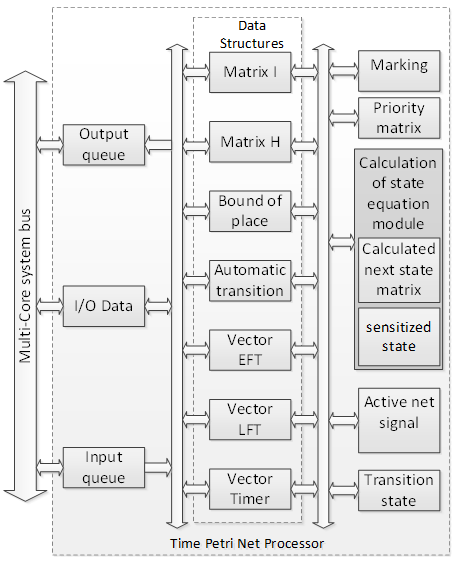
\includegraphics[width=0.95\linewidth]{time_petri_nets_processor}
        \caption{Time Petri Nets Processor}
        \label{fig:time_petri_nets_processor}
    \end{figure}
    
    The output queue has a similar structure, but its function is to communicate to the threads those 
	firings that have been resolved.
	
	The data I/O module manages the access of the cores to the matrixes and vectors that program the 
	system. The module manages the access of the cores to the matrixes and vectors that program the system. 
	
	The matrixes and vectors described in the equation of state are the system program. This allows 
	us to program the processor directly from the Time Petri Net.
	
    Here we have added the inhibitor arcs matrix and the vector indicating the maximum number of tokens 
    in the places. This terms are not present in the state equations shown in this work but you can 
    consult the work\cite{paperProcesador}.\\
    
    The module in charge of solving the state equation of the Petri has the following responsibilities:
	\begin{enumerate}
  		\item Calculating the new state that would result from each transition firing only once, thereby 
  		generating a number of vectors calculated states equal to the number of transitions. Then, 
  		these vectors are stored. This is performed by subtracting the current state parallel to each 
  		column of $I^-$ and storing all resulting vectors, which will be evaluated to determine if 
  		the new state that each transition would produce is valid. This operation is performed whenever 
  		you change the time Petri Nets Processor status (current marking vector).
  		\item Determine which transition is sensitized. To do this, take all vectors calculated in 
  		step 1 and verify that there is no place to have a negative marking and neither exceeding the 
  		limit  of tokens it \footnotemark can hold.
  		\footnotetext{It is noted that this is a weak bound, since the marks in the squares are incremented 
	in step 4 and the limit is checked in step 2. This simplification facilitates hardware implementation.}
  		\item It starts or stops the timer. If a transition t has been sensitized and $Timer_t=0$ 
  		starts $Timer_t$, if $Timer_t\neq0$ does nothing.
  		\item Firing of one transition. Transitions that meet:
  		\begin{equation*}
			Vector EFT \leq Vector Timer_t \leq Vector LFT
		\end{equation*}				
		The transitions that meet that condition and have received one firing from input queue or 
		the firing programmed as automatic (which form a set of available firings).
		
		From that set, the firing with highest priority is selected and the transition is executed.
		
		According the executed transition, the state vector is actualized and the $Timer_t$  is 
		resetted to zero.
		\item Execute the steps 1, 2, 3 and 4 as a continuous cycle.\\
	\end{enumerate}	
	
	
	
	The system also has a unit that detects when no transition is sensitized and none $Timer_t$ 
	is higher than $LFT_t$. When this happens, the system generates an interruption notifying that 
	the system has finished its execution or is deadlocked. This feature is very useful to verify 
	the operation of the design and implementation of the system.
	
    